\chapter{Conception g\'enerale du projet}

\section{Introduction}
Ce chapitre est consacr\'e \`a la conception g\'en\'erale du projet. Apr\`es la d\'efinition des besoins fonctionnels et non fonctionnels, nous allons passer \`a la conception de l'architecture fonctionnelle qui repr\'esente une vue globale de la solution avec une prise en consid\'eration du besoin de la modularit\'e. 

\section{Conception g\'en\'erale}

\subsection{Architecture globale du syst\`eme}

Apr\`es la d\'efinition des besoins fonctionnels et non fonctionnels, nous avons pass\'e \`a la conception de l'architecture fonctionnelle qui repr\'esente une vue globale de la solution avec une prise en consid\'eration du besoin de la modularit\'e. Comme le montre la figure suivante :

\begin{figure}[h]
	\center{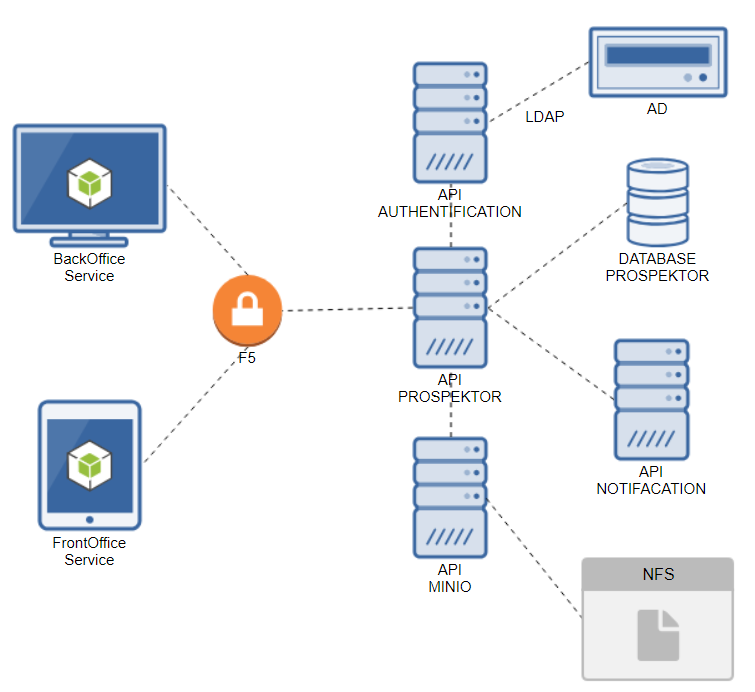
\includegraphics[width=\textwidth]{Figures/architecture.PNG}}
	\caption{\label{fig:my-label} Architecture du syst\`eme}
\end{figure}

Cette architecture est d\'efinie pour les prospecteurs et les exploitant qui vont utiliser notre application mobile.

architecture du syst\`eme est compose par:
\begin{itemize}
\item \textbf{F5 VPN} : utilise le protocole Secure Sockets Layer, une technologie d'authentification et de cryptage int\'egr\'ee \`a chaque navigateur Web, pour cr\'eer une connexion s\'ecuris\'ee et crypt\'ee sur un r\'eseau moins s\'ecuris\'e, comme Internet.
\item \textbf{MINIO} : vous permet d'utiliser un seul NAS (comme NFS, GlusterFS et d'autres systèmes de fichiers distribu\'es) en tant que syst\`eme de stockage pour plusieurs serveurs MinIO. La synchronisation entre les serveurs MinIO est prise en charge par la conception.
\item \gls{AD} est un syst\`eme bas\'e sur une base de donn\'ees qui fournit une authentification, un annuaire, une strat\'egie et d'autres services dans un environnement Windows.
\item \gls{LDAP} est un protocole d'application permettant d'interroger et de modifier des \'el\'ements dans des fournisseurs de services d'annuaire tels qu'Active Directory, qui prend en charge une forme LDAP.
\item \gls{NFS}, litt\'eralement système de fichiers en r\'eseau, est \`a l'origine un protocole qui permet \`a un ordinateur d'acc\'eder via un r\'eseau \`a des fichiers distants.
\end{itemize}

\section{\gls{ERD}}
Un certain nombre de techniques de mod\'elisation de donnd\'ees sont utilisd\'ees aujourd'hui. L'un des plus courants est le diagramme de relation d'entitd\'e (\gls{ERD}). Plusieurs notations \gls{ERD} sont disponibles. Nous avons utilis\'e la notation du Crow's Foot.

La \textbf{cardinalit\'e} et la \textbf{modalit\'e} sont les indicateurs des r\`egles de gestion entourant une relation. La cardinalit\'e fait r\'ef\'erence au nombre maximum de fois qu'une instance d'une entit\'e peut \^etre associ\'ee \`a des instances de l'entit\'e associ\'ee. La modalit\'e fait r\'ef\'erence au nombre minimum de fois qu'une instance d'une entit\'e peut \^etre associ\'ee \`a une instance de l'entit\'e associ\'ee.

\begin{table}[H]
\begin{center}
\begin{tabular}{ ll }
\hline Symbole & cardinalit\'e \\ \hline
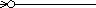
\includegraphics[width=0.2\textwidth]{Figures/0+.png}
& z\'ero ou plus \\
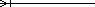
\includegraphics[width=0.2\textwidth]{Figures/1+.png}
& 1 ou plus \\
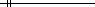
\includegraphics[width=0.2\textwidth]{Figures/11.png}
& 1 et seulement 1 \\
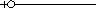
\includegraphics[width=0.2\textwidth]{Figures/01.png}
& z\'ero ou 1
\end{tabular}
\caption{Cardinalit\'e du Crow's Foot}
\end{center}
\end{table}

\begin{figure}[H]
	\center{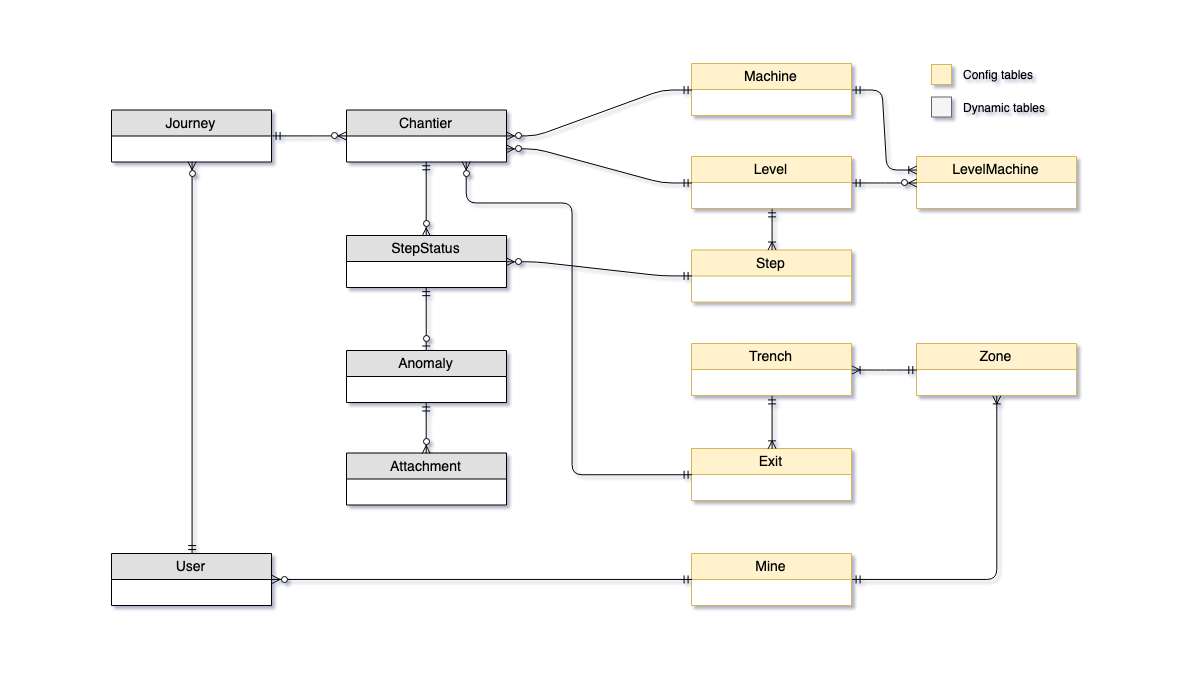
\includegraphics[width=\textwidth]{Figures/crowsfeet.PNG}}
	\caption{\label{fig:my-label} Diagramme de Crow's Foot}
\end{figure}

